\documentclass[twoside]{book}

% Packages required by doxygen
\usepackage{fixltx2e}
\usepackage{calc}
\usepackage{doxygen}
\usepackage[export]{adjustbox} % also loads graphicx
\usepackage{graphicx}
\usepackage[utf8]{inputenc}
\usepackage{makeidx}
\usepackage{multicol}
\usepackage{multirow}
\PassOptionsToPackage{warn}{textcomp}
\usepackage{textcomp}
\usepackage[nointegrals]{wasysym}
\usepackage[table]{xcolor}

% Font selection
\usepackage[T1]{fontenc}
\usepackage[scaled=.90]{helvet}
\usepackage{courier}
\usepackage{amssymb}
\usepackage{sectsty}
\renewcommand{\familydefault}{\sfdefault}
\allsectionsfont{%
  \fontseries{bc}\selectfont%
  \color{darkgray}%
}
\renewcommand{\DoxyLabelFont}{%
  \fontseries{bc}\selectfont%
  \color{darkgray}%
}
\newcommand{\+}{\discretionary{\mbox{\scriptsize$\hookleftarrow$}}{}{}}

% Page & text layout
\usepackage{geometry}
\geometry{%
  a4paper,%
  top=2.5cm,%
  bottom=2.5cm,%
  left=2.5cm,%
  right=2.5cm%
}
\tolerance=750
\hfuzz=15pt
\hbadness=750
\setlength{\emergencystretch}{15pt}
\setlength{\parindent}{0cm}
\setlength{\parskip}{3ex plus 2ex minus 2ex}
\makeatletter
\renewcommand{\paragraph}{%
  \@startsection{paragraph}{4}{0ex}{-1.0ex}{1.0ex}{%
    \normalfont\normalsize\bfseries\SS@parafont%
  }%
}
\renewcommand{\subparagraph}{%
  \@startsection{subparagraph}{5}{0ex}{-1.0ex}{1.0ex}{%
    \normalfont\normalsize\bfseries\SS@subparafont%
  }%
}
\makeatother

% Headers & footers
\usepackage{fancyhdr}
\pagestyle{fancyplain}
\fancyhead[LE]{\fancyplain{}{\bfseries\thepage}}
\fancyhead[CE]{\fancyplain{}{}}
\fancyhead[RE]{\fancyplain{}{\bfseries\leftmark}}
\fancyhead[LO]{\fancyplain{}{\bfseries\rightmark}}
\fancyhead[CO]{\fancyplain{}{}}
\fancyhead[RO]{\fancyplain{}{\bfseries\thepage}}
\fancyfoot[LE]{\fancyplain{}{}}
\fancyfoot[CE]{\fancyplain{}{}}
\fancyfoot[RE]{\fancyplain{}{\bfseries\scriptsize Generated by Doxygen }}
\fancyfoot[LO]{\fancyplain{}{\bfseries\scriptsize Generated by Doxygen }}
\fancyfoot[CO]{\fancyplain{}{}}
\fancyfoot[RO]{\fancyplain{}{}}
\renewcommand{\footrulewidth}{0.4pt}
\renewcommand{\chaptermark}[1]{%
  \markboth{#1}{}%
}
\renewcommand{\sectionmark}[1]{%
  \markright{\thesection\ #1}%
}

% Indices & bibliography
\usepackage{natbib}
\usepackage[titles]{tocloft}
\setcounter{tocdepth}{3}
\setcounter{secnumdepth}{5}
\makeindex

% Hyperlinks (required, but should be loaded last)
\usepackage{ifpdf}
\ifpdf
  \usepackage[pdftex,pagebackref=true]{hyperref}
\else
  \usepackage[ps2pdf,pagebackref=true]{hyperref}
\fi
\hypersetup{%
  colorlinks=true,%
  linkcolor=blue,%
  citecolor=blue,%
  unicode%
}

% Custom commands
\newcommand{\clearemptydoublepage}{%
  \newpage{\pagestyle{empty}\cleardoublepage}%
}

\usepackage{caption}
\captionsetup{labelsep=space,justification=centering,font={bf},singlelinecheck=off,skip=4pt,position=top}

%===== C O N T E N T S =====

\begin{document}

% Titlepage & ToC
\hypersetup{pageanchor=false,
             bookmarksnumbered=true,
             pdfencoding=unicode
            }
\pagenumbering{alph}
\begin{titlepage}
\vspace*{7cm}
\begin{center}%
{\Large Assignment 2 }\\
\vspace*{1cm}
{\large Generated by Doxygen 1.8.13}\\
\end{center}
\end{titlepage}
\clearemptydoublepage
\pagenumbering{roman}
\tableofcontents
\clearemptydoublepage
\pagenumbering{arabic}
\hypersetup{pageanchor=true}

%--- Begin generated contents ---
\chapter{Hierarchical Index}
\section{Class Hierarchy}
This inheritance list is sorted roughly, but not completely, alphabetically\+:\begin{DoxyCompactList}
\item \contentsline{section}{A\+A\+Lst.\+A\+A\+Lst}{\pageref{class_a_a_lst_1_1_a_a_lst}}{}
\item \contentsline{section}{D\+Cap\+A\+Lst.\+D\+Cap\+A\+Lst}{\pageref{class_d_cap_a_lst_1_1_d_cap_a_lst}}{}
\item \contentsline{section}{S\+A\+Lst.\+S\+A\+Lst}{\pageref{class_s_a_lst_1_1_s_a_lst}}{}
\item \contentsline{section}{Seq\+A\+D\+T.\+Seq\+A\+DT}{\pageref{class_seq_a_d_t_1_1_seq_a_d_t}}{}
\item Enum\begin{DoxyCompactList}
\item \contentsline{section}{Stdnt\+Alloc\+Types.\+DeptT}{\pageref{class_stdnt_alloc_types_1_1_dept_t}}{}
\item \contentsline{section}{Stdnt\+Alloc\+Types.\+GenT}{\pageref{class_stdnt_alloc_types_1_1_gen_t}}{}
\end{DoxyCompactList}
\item Named\+Tuple\begin{DoxyCompactList}
\item \contentsline{section}{Stdnt\+Alloc\+Types.\+S\+InfoT}{\pageref{class_stdnt_alloc_types_1_1_s_info_t}}{}
\end{DoxyCompactList}
\end{DoxyCompactList}

\chapter{Class Index}
\section{Class List}
Here are the classes, structs, unions and interfaces with brief descriptions\+:\begin{DoxyCompactList}
\item\contentsline{section}{\hyperlink{class_a_a_lst_1_1_a_a_lst}{A\+A\+Lst.\+A\+A\+Lst} \\*An abstract data type containing engineering departments and the students allocated into them }{\pageref{class_a_a_lst_1_1_a_a_lst}}{}
\item\contentsline{section}{\hyperlink{class_d_cap_a_lst_1_1_d_cap_a_lst}{D\+Cap\+A\+Lst.\+D\+Cap\+A\+Lst} \\*An abstract data type containing the capacities of engineering departments as a list }{\pageref{class_d_cap_a_lst_1_1_d_cap_a_lst}}{}
\item\contentsline{section}{\hyperlink{class_stdnt_alloc_types_1_1_dept_t}{Stdnt\+Alloc\+Types.\+DeptT} \\*An Enumerated type of possible engineering departments }{\pageref{class_stdnt_alloc_types_1_1_dept_t}}{}
\item\contentsline{section}{\hyperlink{class_stdnt_alloc_types_1_1_gen_t}{Stdnt\+Alloc\+Types.\+GenT} \\*An Enumerated type of possible genders }{\pageref{class_stdnt_alloc_types_1_1_gen_t}}{}
\item\contentsline{section}{\hyperlink{class_s_a_lst_1_1_s_a_lst}{S\+A\+Lst.\+S\+A\+Lst} \\*An abstract data type of all first year engineerng students }{\pageref{class_s_a_lst_1_1_s_a_lst}}{}
\item\contentsline{section}{\hyperlink{class_seq_a_d_t_1_1_seq_a_d_t}{Seq\+A\+D\+T.\+Seq\+A\+DT} \\*An abstract data type that represents a sequence of values }{\pageref{class_seq_a_d_t_1_1_seq_a_d_t}}{}
\item\contentsline{section}{\hyperlink{class_stdnt_alloc_types_1_1_s_info_t}{Stdnt\+Alloc\+Types.\+S\+InfoT} \\*A Named\+Tuple used to represent a student }{\pageref{class_stdnt_alloc_types_1_1_s_info_t}}{}
\end{DoxyCompactList}

\chapter{File Index}
\section{File List}
Here is a list of all documented files with brief descriptions\+:\begin{DoxyCompactList}
\item\contentsline{section}{src/\hyperlink{_a_a_lst_8py}{A\+A\+Lst.\+py} \\*Allocation Association List Module }{\pageref{_a_a_lst_8py}}{}
\item\contentsline{section}{src/\hyperlink{_d_cap_a_lst_8py}{D\+Cap\+A\+Lst.\+py} \\*Department Capacity Association List }{\pageref{_d_cap_a_lst_8py}}{}
\item\contentsline{section}{src/\hyperlink{_read_8py}{Read.\+py} \\*Read }{\pageref{_read_8py}}{}
\item\contentsline{section}{src/\hyperlink{_s_a_lst_8py}{S\+A\+Lst.\+py} \\*Student Association List }{\pageref{_s_a_lst_8py}}{}
\item\contentsline{section}{src/\hyperlink{_seq_a_d_t_8py}{Seq\+A\+D\+T.\+py} \\*Sequence A\+DT }{\pageref{_seq_a_d_t_8py}}{}
\item\contentsline{section}{src/\hyperlink{_stdnt_alloc_types_8py}{Stdnt\+Alloc\+Types.\+py} \\*Student Allocation Types }{\pageref{_stdnt_alloc_types_8py}}{}
\end{DoxyCompactList}

\chapter{Class Documentation}
\hypertarget{class_a_a_lst_1_1_a_a_lst}{}\section{A\+A\+Lst.\+A\+A\+Lst Class Reference}
\label{class_a_a_lst_1_1_a_a_lst}\index{A\+A\+Lst.\+A\+A\+Lst@{A\+A\+Lst.\+A\+A\+Lst}}


An abstract data type containing engineering departments and the students allocated into them.  


\subsection*{Static Public Member Functions}
\begin{DoxyCompactItemize}
\item 
def \hyperlink{class_a_a_lst_1_1_a_a_lst_ade2ae95f7a0e7ad568b8fdcccdc18556}{init} ()
\begin{DoxyCompactList}\small\item\em Initiazlies the \hyperlink{class_a_a_lst_1_1_a_a_lst}{A\+A\+Lst}. \end{DoxyCompactList}\item 
def \hyperlink{class_a_a_lst_1_1_a_a_lst_ac43ad5933af821d0763f532a50d83745}{add\+\_\+stdnt}
\item 
def \hyperlink{class_a_a_lst_1_1_a_a_lst_ab3b9d7b152fbc79215fc572b253ce239}{lst\+\_\+alloc}
\item 
def \hyperlink{class_a_a_lst_1_1_a_a_lst_adc3cda4fa36f60abdf614964290b98f9}{num\+\_\+alloc}
\end{DoxyCompactItemize}


\subsection{Detailed Description}
An abstract data type containing engineering departments and the students allocated into them. 

\subsection{Member Function Documentation}
\mbox{\Hypertarget{class_a_a_lst_1_1_a_a_lst_ac43ad5933af821d0763f532a50d83745}\label{class_a_a_lst_1_1_a_a_lst_ac43ad5933af821d0763f532a50d83745}} 
\index{A\+A\+Lst\+::\+A\+A\+Lst@{A\+A\+Lst\+::\+A\+A\+Lst}!add\+\_\+stdnt@{add\+\_\+stdnt}}
\index{add\+\_\+stdnt@{add\+\_\+stdnt}!A\+A\+Lst\+::\+A\+A\+Lst@{A\+A\+Lst\+::\+A\+A\+Lst}}
\subsubsection{\texorpdfstring{add\+\_\+stdnt()}{add\_stdnt()}}
{\footnotesize\ttfamily def A\+A\+Lst.\+A\+A\+Lst.\+add\+\_\+stdnt (\begin{DoxyParamCaption}\item[{}]{dep }\end{DoxyParamCaption})\hspace{0.3cm}{\ttfamily [static]}}

add\+\_\+stdnt adds a student to a specific department 
\begin{DoxyParams}{Parameters}
{\em dep} & A department of type \hyperlink{class_stdnt_alloc_types_1_1_dept_t}{Stdnt\+Alloc\+Types.\+DeptT} \\
\hline
{\em m} & A string representing the students macid \\
\hline
\end{DoxyParams}
\mbox{\Hypertarget{class_a_a_lst_1_1_a_a_lst_ade2ae95f7a0e7ad568b8fdcccdc18556}\label{class_a_a_lst_1_1_a_a_lst_ade2ae95f7a0e7ad568b8fdcccdc18556}} 
\index{A\+A\+Lst\+::\+A\+A\+Lst@{A\+A\+Lst\+::\+A\+A\+Lst}!init@{init}}
\index{init@{init}!A\+A\+Lst\+::\+A\+A\+Lst@{A\+A\+Lst\+::\+A\+A\+Lst}}
\subsubsection{\texorpdfstring{init()}{init()}}
{\footnotesize\ttfamily def A\+A\+Lst.\+A\+A\+Lst.\+init (\begin{DoxyParamCaption}{ }\end{DoxyParamCaption})\hspace{0.3cm}{\ttfamily [static]}}



Initiazlies the \hyperlink{class_a_a_lst_1_1_a_a_lst}{A\+A\+Lst}. 

The list is initialized with each department and an empty list of students for each department. \mbox{\Hypertarget{class_a_a_lst_1_1_a_a_lst_ab3b9d7b152fbc79215fc572b253ce239}\label{class_a_a_lst_1_1_a_a_lst_ab3b9d7b152fbc79215fc572b253ce239}} 
\index{A\+A\+Lst\+::\+A\+A\+Lst@{A\+A\+Lst\+::\+A\+A\+Lst}!lst\+\_\+alloc@{lst\+\_\+alloc}}
\index{lst\+\_\+alloc@{lst\+\_\+alloc}!A\+A\+Lst\+::\+A\+A\+Lst@{A\+A\+Lst\+::\+A\+A\+Lst}}
\subsubsection{\texorpdfstring{lst\+\_\+alloc()}{lst\_alloc()}}
{\footnotesize\ttfamily def A\+A\+Lst.\+A\+A\+Lst.\+lst\+\_\+alloc (\begin{DoxyParamCaption}\item[{}]{d }\end{DoxyParamCaption})\hspace{0.3cm}{\ttfamily [static]}}

lst\+\_\+alloc returns a list of students in a specific department 
\begin{DoxyParams}{Parameters}
{\em d} & A department of type \hyperlink{class_stdnt_alloc_types_1_1_dept_t}{Stdnt\+Alloc\+Types.\+DeptT} \\
\hline
\end{DoxyParams}
\begin{DoxyReturn}{Returns}
A list of strings where each string is a macid 
\end{DoxyReturn}
\mbox{\Hypertarget{class_a_a_lst_1_1_a_a_lst_adc3cda4fa36f60abdf614964290b98f9}\label{class_a_a_lst_1_1_a_a_lst_adc3cda4fa36f60abdf614964290b98f9}} 
\index{A\+A\+Lst\+::\+A\+A\+Lst@{A\+A\+Lst\+::\+A\+A\+Lst}!num\+\_\+alloc@{num\+\_\+alloc}}
\index{num\+\_\+alloc@{num\+\_\+alloc}!A\+A\+Lst\+::\+A\+A\+Lst@{A\+A\+Lst\+::\+A\+A\+Lst}}
\subsubsection{\texorpdfstring{num\+\_\+alloc()}{num\_alloc()}}
{\footnotesize\ttfamily def A\+A\+Lst.\+A\+A\+Lst.\+num\+\_\+alloc (\begin{DoxyParamCaption}\item[{}]{d }\end{DoxyParamCaption})\hspace{0.3cm}{\ttfamily [static]}}

num\+\_\+alloc returns the number of students in a department 
\begin{DoxyParams}{Parameters}
{\em d} & A department of type \hyperlink{class_stdnt_alloc_types_1_1_dept_t}{Stdnt\+Alloc\+Types.\+DeptT} \\
\hline
\end{DoxyParams}
\begin{DoxyReturn}{Returns}
A integer representing the number of students in a department 
\end{DoxyReturn}


The documentation for this class was generated from the following file\+:\begin{DoxyCompactItemize}
\item 
src/\hyperlink{_a_a_lst_8py}{A\+A\+Lst.\+py}\end{DoxyCompactItemize}

\hypertarget{class_d_cap_a_lst_1_1_d_cap_a_lst}{}\section{D\+Cap\+A\+Lst.\+D\+Cap\+A\+Lst Class Reference}
\label{class_d_cap_a_lst_1_1_d_cap_a_lst}\index{D\+Cap\+A\+Lst.\+D\+Cap\+A\+Lst@{D\+Cap\+A\+Lst.\+D\+Cap\+A\+Lst}}


An abstract data type containing the capacities of engineering departments as a list.  


\subsection*{Static Public Member Functions}
\begin{DoxyCompactItemize}
\item 
\mbox{\Hypertarget{class_d_cap_a_lst_1_1_d_cap_a_lst_aaed5d536e93c43a53eca6c75faa64d2e}\label{class_d_cap_a_lst_1_1_d_cap_a_lst_aaed5d536e93c43a53eca6c75faa64d2e}} 
def \hyperlink{class_d_cap_a_lst_1_1_d_cap_a_lst_aaed5d536e93c43a53eca6c75faa64d2e}{init} ()
\begin{DoxyCompactList}\small\item\em Initializes the Department Capacity List to be empty. \end{DoxyCompactList}\item 
def \hyperlink{class_d_cap_a_lst_1_1_d_cap_a_lst_a7ae2713aa4cf52277bf95d345033aef1}{add}
\begin{DoxyCompactList}\small\item\em Adds a department and its capacity to the list. \end{DoxyCompactList}\item 
def \hyperlink{class_d_cap_a_lst_1_1_d_cap_a_lst_a8c708603e65c31aaf03449c3e449a900}{remove}
\begin{DoxyCompactList}\small\item\em Removes a department and its capacity from the list \end{DoxyCompactList}\item 
def \hyperlink{class_d_cap_a_lst_1_1_d_cap_a_lst_a1544d1dd5a4da06d12379ff2b752b5fc}{elm}
\begin{DoxyCompactList}\small\item\em elm checks if a department has been added \end{DoxyCompactList}\item 
def \hyperlink{class_d_cap_a_lst_1_1_d_cap_a_lst_a60327f8162913725028ca07da0d14e69}{capacity}
\begin{DoxyCompactList}\small\item\em capacity returns the capacity of a department \end{DoxyCompactList}\end{DoxyCompactItemize}


\subsection{Detailed Description}
An abstract data type containing the capacities of engineering departments as a list. 

\subsection{Member Function Documentation}
\mbox{\Hypertarget{class_d_cap_a_lst_1_1_d_cap_a_lst_a7ae2713aa4cf52277bf95d345033aef1}\label{class_d_cap_a_lst_1_1_d_cap_a_lst_a7ae2713aa4cf52277bf95d345033aef1}} 
\index{D\+Cap\+A\+Lst\+::\+D\+Cap\+A\+Lst@{D\+Cap\+A\+Lst\+::\+D\+Cap\+A\+Lst}!add@{add}}
\index{add@{add}!D\+Cap\+A\+Lst\+::\+D\+Cap\+A\+Lst@{D\+Cap\+A\+Lst\+::\+D\+Cap\+A\+Lst}}
\subsubsection{\texorpdfstring{add()}{add()}}
{\footnotesize\ttfamily def D\+Cap\+A\+Lst.\+D\+Cap\+A\+Lst.\+add (\begin{DoxyParamCaption}\item[{}]{d }\end{DoxyParamCaption})\hspace{0.3cm}{\ttfamily [static]}}



Adds a department and its capacity to the list. 


\begin{DoxyExceptions}{Exceptions}
{\em throws} & Key\+Error if the given department has been added before \\
\hline
\end{DoxyExceptions}

\begin{DoxyParams}{Parameters}
{\em d} & A department of type \hyperlink{class_stdnt_alloc_types_1_1_dept_t}{Stdnt\+Alloc\+Types.\+DeptT} \\
\hline
{\em n} & An integer representing the capacity of the department (d parameter) \\
\hline
\end{DoxyParams}
\mbox{\Hypertarget{class_d_cap_a_lst_1_1_d_cap_a_lst_a60327f8162913725028ca07da0d14e69}\label{class_d_cap_a_lst_1_1_d_cap_a_lst_a60327f8162913725028ca07da0d14e69}} 
\index{D\+Cap\+A\+Lst\+::\+D\+Cap\+A\+Lst@{D\+Cap\+A\+Lst\+::\+D\+Cap\+A\+Lst}!capacity@{capacity}}
\index{capacity@{capacity}!D\+Cap\+A\+Lst\+::\+D\+Cap\+A\+Lst@{D\+Cap\+A\+Lst\+::\+D\+Cap\+A\+Lst}}
\subsubsection{\texorpdfstring{capacity()}{capacity()}}
{\footnotesize\ttfamily def D\+Cap\+A\+Lst.\+D\+Cap\+A\+Lst.\+capacity (\begin{DoxyParamCaption}\item[{}]{d }\end{DoxyParamCaption})\hspace{0.3cm}{\ttfamily [static]}}



capacity returns the capacity of a department 


\begin{DoxyExceptions}{Exceptions}
{\em throws} & Key\+Error if the department given is not in \hyperlink{class_d_cap_a_lst_1_1_d_cap_a_lst}{D\+Cap\+A\+Lst} \\
\hline
\end{DoxyExceptions}

\begin{DoxyParams}{Parameters}
{\em d} & A department of type \hyperlink{class_stdnt_alloc_types_1_1_dept_t}{Stdnt\+Alloc\+Types.\+DeptT} \\
\hline
\end{DoxyParams}
\begin{DoxyReturn}{Returns}
An integer representing the capacity of the department given as a parameter. 
\end{DoxyReturn}
\mbox{\Hypertarget{class_d_cap_a_lst_1_1_d_cap_a_lst_a1544d1dd5a4da06d12379ff2b752b5fc}\label{class_d_cap_a_lst_1_1_d_cap_a_lst_a1544d1dd5a4da06d12379ff2b752b5fc}} 
\index{D\+Cap\+A\+Lst\+::\+D\+Cap\+A\+Lst@{D\+Cap\+A\+Lst\+::\+D\+Cap\+A\+Lst}!elm@{elm}}
\index{elm@{elm}!D\+Cap\+A\+Lst\+::\+D\+Cap\+A\+Lst@{D\+Cap\+A\+Lst\+::\+D\+Cap\+A\+Lst}}
\subsubsection{\texorpdfstring{elm()}{elm()}}
{\footnotesize\ttfamily def D\+Cap\+A\+Lst.\+D\+Cap\+A\+Lst.\+elm (\begin{DoxyParamCaption}\item[{}]{d }\end{DoxyParamCaption})\hspace{0.3cm}{\ttfamily [static]}}



elm checks if a department has been added 


\begin{DoxyParams}{Parameters}
{\em d} & A department of type \hyperlink{class_stdnt_alloc_types_1_1_dept_t}{Stdnt\+Alloc\+Types.\+DeptT} \\
\hline
\end{DoxyParams}
\begin{DoxyReturn}{Returns}
True if the department has been added, otherwise False 
\end{DoxyReturn}
\mbox{\Hypertarget{class_d_cap_a_lst_1_1_d_cap_a_lst_a8c708603e65c31aaf03449c3e449a900}\label{class_d_cap_a_lst_1_1_d_cap_a_lst_a8c708603e65c31aaf03449c3e449a900}} 
\index{D\+Cap\+A\+Lst\+::\+D\+Cap\+A\+Lst@{D\+Cap\+A\+Lst\+::\+D\+Cap\+A\+Lst}!remove@{remove}}
\index{remove@{remove}!D\+Cap\+A\+Lst\+::\+D\+Cap\+A\+Lst@{D\+Cap\+A\+Lst\+::\+D\+Cap\+A\+Lst}}
\subsubsection{\texorpdfstring{remove()}{remove()}}
{\footnotesize\ttfamily def D\+Cap\+A\+Lst.\+D\+Cap\+A\+Lst.\+remove (\begin{DoxyParamCaption}\item[{}]{d }\end{DoxyParamCaption})\hspace{0.3cm}{\ttfamily [static]}}



Removes a department and its capacity from the list 


\begin{DoxyExceptions}{Exceptions}
{\em throws} & Key\+Error if the given department is not in \hyperlink{class_d_cap_a_lst_1_1_d_cap_a_lst}{D\+Cap\+A\+Lst} \\
\hline
\end{DoxyExceptions}

\begin{DoxyParams}{Parameters}
{\em d} & A department of type \hyperlink{class_stdnt_alloc_types_1_1_dept_t}{Stdnt\+Alloc\+Types.\+DeptT} to be removed \\
\hline
\end{DoxyParams}


The documentation for this class was generated from the following file\+:\begin{DoxyCompactItemize}
\item 
src/\hyperlink{_d_cap_a_lst_8py}{D\+Cap\+A\+Lst.\+py}\end{DoxyCompactItemize}

\hypertarget{class_stdnt_alloc_types_1_1_dept_t}{}\section{Stdnt\+Alloc\+Types.\+DeptT Class Reference}
\label{class_stdnt_alloc_types_1_1_dept_t}\index{Stdnt\+Alloc\+Types.\+DeptT@{Stdnt\+Alloc\+Types.\+DeptT}}


An Enumerated type of possible engineering departments.  


Inheritance diagram for Stdnt\+Alloc\+Types.\+DeptT\+:\begin{figure}[H]
\begin{center}
\leavevmode
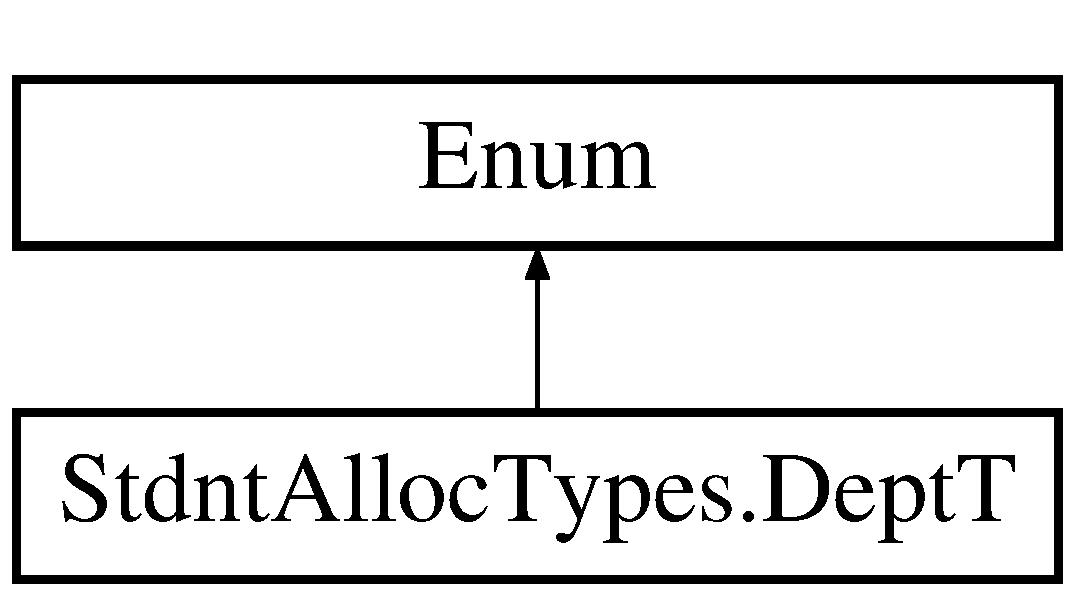
\includegraphics[height=2.000000cm]{class_stdnt_alloc_types_1_1_dept_t}
\end{center}
\end{figure}
\subsection*{Static Public Attributes}
\begin{DoxyCompactItemize}
\item 
\mbox{\Hypertarget{class_stdnt_alloc_types_1_1_dept_t_a578b321a2301c134046d1b7a435840f4}\label{class_stdnt_alloc_types_1_1_dept_t_a578b321a2301c134046d1b7a435840f4}} 
string {\bfseries civil} = \char`\"{}civil\char`\"{}
\item 
\mbox{\Hypertarget{class_stdnt_alloc_types_1_1_dept_t_a00f9d4c89adaac8cb29fb9b1fb49c6b6}\label{class_stdnt_alloc_types_1_1_dept_t_a00f9d4c89adaac8cb29fb9b1fb49c6b6}} 
string {\bfseries chemical} = \char`\"{}chemical\char`\"{}
\item 
\mbox{\Hypertarget{class_stdnt_alloc_types_1_1_dept_t_a1073a0bacdf2538b83b6cc649d1281e5}\label{class_stdnt_alloc_types_1_1_dept_t_a1073a0bacdf2538b83b6cc649d1281e5}} 
string {\bfseries electrical} = \char`\"{}electrical\char`\"{}
\item 
\mbox{\Hypertarget{class_stdnt_alloc_types_1_1_dept_t_a8f0286f2c8bdfa90f2e96d3968872bc5}\label{class_stdnt_alloc_types_1_1_dept_t_a8f0286f2c8bdfa90f2e96d3968872bc5}} 
string {\bfseries mechanical} = \char`\"{}mechanical\char`\"{}
\item 
\mbox{\Hypertarget{class_stdnt_alloc_types_1_1_dept_t_a321e6a6c4a7f6177ab04d66966666405}\label{class_stdnt_alloc_types_1_1_dept_t_a321e6a6c4a7f6177ab04d66966666405}} 
string {\bfseries software} = \char`\"{}software\char`\"{}
\item 
\mbox{\Hypertarget{class_stdnt_alloc_types_1_1_dept_t_a89e5ca2915bbade29c54a4cb3c5d80a1}\label{class_stdnt_alloc_types_1_1_dept_t_a89e5ca2915bbade29c54a4cb3c5d80a1}} 
string {\bfseries materials} = \char`\"{}materials\char`\"{}
\item 
\mbox{\Hypertarget{class_stdnt_alloc_types_1_1_dept_t_a150e6c3b5f94d1fb6b70be0c4f8848aa}\label{class_stdnt_alloc_types_1_1_dept_t_a150e6c3b5f94d1fb6b70be0c4f8848aa}} 
string {\bfseries engphys} = \char`\"{}engphys\char`\"{}
\end{DoxyCompactItemize}


\subsection{Detailed Description}
An Enumerated type of possible engineering departments. 

The documentation for this class was generated from the following file\+:\begin{DoxyCompactItemize}
\item 
src/\hyperlink{_stdnt_alloc_types_8py}{Stdnt\+Alloc\+Types.\+py}\end{DoxyCompactItemize}

\hypertarget{class_stdnt_alloc_types_1_1_gen_t}{}\section{Stdnt\+Alloc\+Types.\+GenT Class Reference}
\label{class_stdnt_alloc_types_1_1_gen_t}\index{Stdnt\+Alloc\+Types.\+GenT@{Stdnt\+Alloc\+Types.\+GenT}}


An Enumerated type of possible genders  


Inheritance diagram for Stdnt\+Alloc\+Types.\+GenT\+:\begin{figure}[H]
\begin{center}
\leavevmode
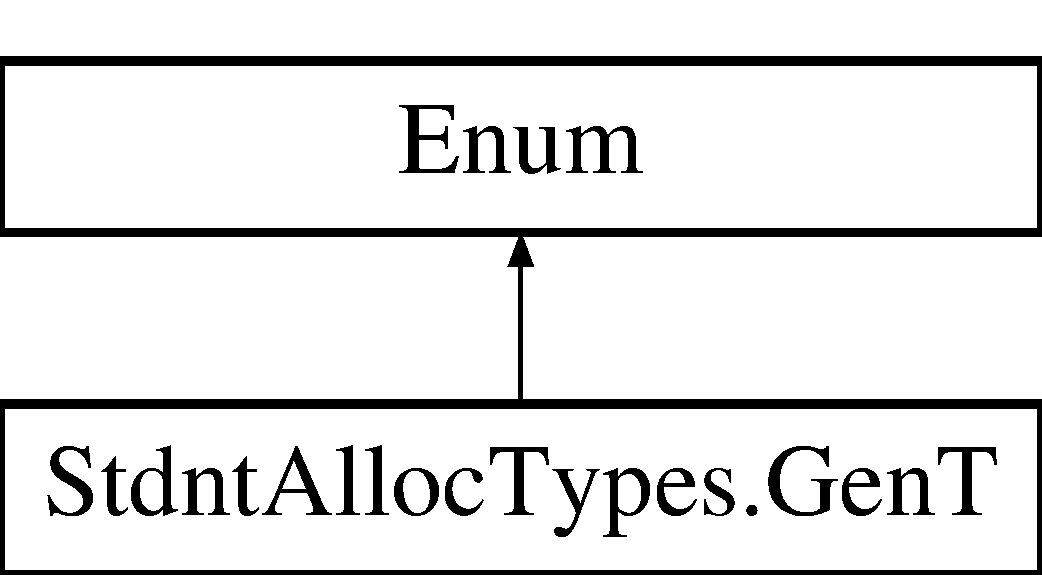
\includegraphics[height=2.000000cm]{class_stdnt_alloc_types_1_1_gen_t}
\end{center}
\end{figure}
\subsection*{Static Public Attributes}
\begin{DoxyCompactItemize}
\item 
\mbox{\Hypertarget{class_stdnt_alloc_types_1_1_gen_t_aeae560b694f78e0f03043f37da016eb4}\label{class_stdnt_alloc_types_1_1_gen_t_aeae560b694f78e0f03043f37da016eb4}} 
string {\bfseries male} = \char`\"{}male\char`\"{}
\item 
\mbox{\Hypertarget{class_stdnt_alloc_types_1_1_gen_t_ad35b4a5d9eb1c3ef88bdd1fcad214d33}\label{class_stdnt_alloc_types_1_1_gen_t_ad35b4a5d9eb1c3ef88bdd1fcad214d33}} 
string {\bfseries female} = \char`\"{}female\char`\"{}
\end{DoxyCompactItemize}


\subsection{Detailed Description}
An Enumerated type of possible genders 

The documentation for this class was generated from the following file\+:\begin{DoxyCompactItemize}
\item 
src/\hyperlink{_stdnt_alloc_types_8py}{Stdnt\+Alloc\+Types.\+py}\end{DoxyCompactItemize}

\hypertarget{class_s_a_lst_1_1_s_a_lst}{}\section{S\+A\+Lst.\+S\+A\+Lst Class Reference}
\label{class_s_a_lst_1_1_s_a_lst}\index{S\+A\+Lst.\+S\+A\+Lst@{S\+A\+Lst.\+S\+A\+Lst}}


An abstract data type of all first year engineerng students.  


\subsection*{Static Public Member Functions}
\begin{DoxyCompactItemize}
\item 
\mbox{\Hypertarget{class_s_a_lst_1_1_s_a_lst_ac0886d79feebf875207b927b6d23a959}\label{class_s_a_lst_1_1_s_a_lst_ac0886d79feebf875207b927b6d23a959}} 
def \hyperlink{class_s_a_lst_1_1_s_a_lst_ac0886d79feebf875207b927b6d23a959}{init} ()
\begin{DoxyCompactList}\small\item\em init initializes the list of students to be empty \end{DoxyCompactList}\item 
def \hyperlink{class_s_a_lst_1_1_s_a_lst_af097359087eff2e52ff94bcf1adfcb65}{add}
\begin{DoxyCompactList}\small\item\em Adds a student into the \hyperlink{class_s_a_lst_1_1_s_a_lst}{S\+A\+Lst}. \end{DoxyCompactList}\item 
def \hyperlink{class_s_a_lst_1_1_s_a_lst_a6c80e47dc1bacbb55188c22cd85af8b6}{remove}
\begin{DoxyCompactList}\small\item\em Removes a student from the \hyperlink{class_s_a_lst_1_1_s_a_lst}{S\+A\+Lst}. \end{DoxyCompactList}\item 
def \hyperlink{class_s_a_lst_1_1_s_a_lst_a400ec4c9364988723f6396b278cebf6a}{elm}
\begin{DoxyCompactList}\small\item\em elm checks if a student is already in the \hyperlink{class_s_a_lst_1_1_s_a_lst}{S\+A\+Lst} \end{DoxyCompactList}\item 
def \hyperlink{class_s_a_lst_1_1_s_a_lst_a036cbb53a35ec5cd293617ca24c522fd}{info}
\begin{DoxyCompactList}\small\item\em returns the information assoaciated with a student \end{DoxyCompactList}\item 
def \hyperlink{class_s_a_lst_1_1_s_a_lst_ac16206cda2affb174b739971b58eb519}{sort}
\begin{DoxyCompactList}\small\item\em Sorts a subset of students based on G\+PA. \end{DoxyCompactList}\item 
def \hyperlink{class_s_a_lst_1_1_s_a_lst_ae6178371d181c6b28be24a8c61b1bab7}{average}
\begin{DoxyCompactList}\small\item\em Computes the average of a particular subset of students. \end{DoxyCompactList}\item 
def \hyperlink{class_s_a_lst_1_1_s_a_lst_a8cdba5b89e936165b3628f52d4e80938}{allocate} ()
\begin{DoxyCompactList}\small\item\em Allocates students in \hyperlink{class_s_a_lst_1_1_s_a_lst}{S\+A\+Lst} into their program \end{DoxyCompactList}\end{DoxyCompactItemize}


\subsection{Detailed Description}
An abstract data type of all first year engineerng students. 

\subsection{Member Function Documentation}
\mbox{\Hypertarget{class_s_a_lst_1_1_s_a_lst_af097359087eff2e52ff94bcf1adfcb65}\label{class_s_a_lst_1_1_s_a_lst_af097359087eff2e52ff94bcf1adfcb65}} 
\index{S\+A\+Lst\+::\+S\+A\+Lst@{S\+A\+Lst\+::\+S\+A\+Lst}!add@{add}}
\index{add@{add}!S\+A\+Lst\+::\+S\+A\+Lst@{S\+A\+Lst\+::\+S\+A\+Lst}}
\subsubsection{\texorpdfstring{add()}{add()}}
{\footnotesize\ttfamily def S\+A\+Lst.\+S\+A\+Lst.\+add (\begin{DoxyParamCaption}\item[{}]{m }\end{DoxyParamCaption})\hspace{0.3cm}{\ttfamily [static]}}



Adds a student into the \hyperlink{class_s_a_lst_1_1_s_a_lst}{S\+A\+Lst}. 


\begin{DoxyExceptions}{Exceptions}
{\em throws} & Key\+Error if the student given has been added before \\
\hline
\end{DoxyExceptions}

\begin{DoxyParams}{Parameters}
{\em m} & A string of a student\textquotesingle{}s macid \\
\hline
{\em i} & Information of a student given with the data type \hyperlink{class_stdnt_alloc_types_1_1_s_info_t}{Stdnt\+Alloc\+Types.\+S\+InfoT} \\
\hline
\end{DoxyParams}
\mbox{\Hypertarget{class_s_a_lst_1_1_s_a_lst_a8cdba5b89e936165b3628f52d4e80938}\label{class_s_a_lst_1_1_s_a_lst_a8cdba5b89e936165b3628f52d4e80938}} 
\index{S\+A\+Lst\+::\+S\+A\+Lst@{S\+A\+Lst\+::\+S\+A\+Lst}!allocate@{allocate}}
\index{allocate@{allocate}!S\+A\+Lst\+::\+S\+A\+Lst@{S\+A\+Lst\+::\+S\+A\+Lst}}
\subsubsection{\texorpdfstring{allocate()}{allocate()}}
{\footnotesize\ttfamily def S\+A\+Lst.\+S\+A\+Lst.\+allocate (\begin{DoxyParamCaption}{ }\end{DoxyParamCaption})\hspace{0.3cm}{\ttfamily [static]}}



Allocates students in \hyperlink{class_s_a_lst_1_1_s_a_lst}{S\+A\+Lst} into their program 

Students are allocated into a department in A\+A\+Lst. Students with free choice are allocated first. The remaining students are allocated in a order based on their G\+PA, a student is allocated into their highest preferred choice that is not full in capacity. 
\begin{DoxyExceptions}{Exceptions}
{\em throws} & Runtime\+Error if all of a student\textquotesingle{}s choices are full. \\
\hline
\end{DoxyExceptions}
\mbox{\Hypertarget{class_s_a_lst_1_1_s_a_lst_ae6178371d181c6b28be24a8c61b1bab7}\label{class_s_a_lst_1_1_s_a_lst_ae6178371d181c6b28be24a8c61b1bab7}} 
\index{S\+A\+Lst\+::\+S\+A\+Lst@{S\+A\+Lst\+::\+S\+A\+Lst}!average@{average}}
\index{average@{average}!S\+A\+Lst\+::\+S\+A\+Lst@{S\+A\+Lst\+::\+S\+A\+Lst}}
\subsubsection{\texorpdfstring{average()}{average()}}
{\footnotesize\ttfamily def S\+A\+Lst.\+S\+A\+Lst.\+average (\begin{DoxyParamCaption}\item[{}]{f }\end{DoxyParamCaption})\hspace{0.3cm}{\ttfamily [static]}}



Computes the average of a particular subset of students. 

The method is given a function that is able to filter a student. The function takes in a student(\+S\+Info\+T) and returns True if they pass the filter. The method will then compute the average G\+PA amongst students who passed the filter. 
\begin{DoxyExceptions}{Exceptions}
{\em throws} & Value\+Error if there are no students that pass the filter function. \\
\hline
\end{DoxyExceptions}

\begin{DoxyParams}{Parameters}
{\em f} & A filtering function that returns a boolean \\
\hline
\end{DoxyParams}
\begin{DoxyReturn}{Returns}
A float representing the average G\+PA amongst a subset of students 
\end{DoxyReturn}
\mbox{\Hypertarget{class_s_a_lst_1_1_s_a_lst_a400ec4c9364988723f6396b278cebf6a}\label{class_s_a_lst_1_1_s_a_lst_a400ec4c9364988723f6396b278cebf6a}} 
\index{S\+A\+Lst\+::\+S\+A\+Lst@{S\+A\+Lst\+::\+S\+A\+Lst}!elm@{elm}}
\index{elm@{elm}!S\+A\+Lst\+::\+S\+A\+Lst@{S\+A\+Lst\+::\+S\+A\+Lst}}
\subsubsection{\texorpdfstring{elm()}{elm()}}
{\footnotesize\ttfamily def S\+A\+Lst.\+S\+A\+Lst.\+elm (\begin{DoxyParamCaption}\item[{}]{m }\end{DoxyParamCaption})\hspace{0.3cm}{\ttfamily [static]}}



elm checks if a student is already in the \hyperlink{class_s_a_lst_1_1_s_a_lst}{S\+A\+Lst} 


\begin{DoxyParams}{Parameters}
{\em m} & A string of a student\textquotesingle{}s macid \\
\hline
\end{DoxyParams}
\begin{DoxyReturn}{Returns}
True if a student is in \hyperlink{class_s_a_lst_1_1_s_a_lst}{S\+A\+Lst}, otherwise False 
\end{DoxyReturn}
\mbox{\Hypertarget{class_s_a_lst_1_1_s_a_lst_a036cbb53a35ec5cd293617ca24c522fd}\label{class_s_a_lst_1_1_s_a_lst_a036cbb53a35ec5cd293617ca24c522fd}} 
\index{S\+A\+Lst\+::\+S\+A\+Lst@{S\+A\+Lst\+::\+S\+A\+Lst}!info@{info}}
\index{info@{info}!S\+A\+Lst\+::\+S\+A\+Lst@{S\+A\+Lst\+::\+S\+A\+Lst}}
\subsubsection{\texorpdfstring{info()}{info()}}
{\footnotesize\ttfamily def S\+A\+Lst.\+S\+A\+Lst.\+info (\begin{DoxyParamCaption}\item[{}]{m }\end{DoxyParamCaption})\hspace{0.3cm}{\ttfamily [static]}}



returns the information assoaciated with a student 


\begin{DoxyExceptions}{Exceptions}
{\em throws} & Key\+Error if the student is not found \\
\hline
\end{DoxyExceptions}

\begin{DoxyParams}{Parameters}
{\em m} & A string of a student\textquotesingle{}s macid \\
\hline
\end{DoxyParams}
\begin{DoxyReturn}{Returns}
A students information with the type \hyperlink{class_stdnt_alloc_types_1_1_s_info_t}{Stdnt\+Alloc\+Types.\+S\+InfoT} 
\end{DoxyReturn}
\mbox{\Hypertarget{class_s_a_lst_1_1_s_a_lst_a6c80e47dc1bacbb55188c22cd85af8b6}\label{class_s_a_lst_1_1_s_a_lst_a6c80e47dc1bacbb55188c22cd85af8b6}} 
\index{S\+A\+Lst\+::\+S\+A\+Lst@{S\+A\+Lst\+::\+S\+A\+Lst}!remove@{remove}}
\index{remove@{remove}!S\+A\+Lst\+::\+S\+A\+Lst@{S\+A\+Lst\+::\+S\+A\+Lst}}
\subsubsection{\texorpdfstring{remove()}{remove()}}
{\footnotesize\ttfamily def S\+A\+Lst.\+S\+A\+Lst.\+remove (\begin{DoxyParamCaption}\item[{}]{m }\end{DoxyParamCaption})\hspace{0.3cm}{\ttfamily [static]}}



Removes a student from the \hyperlink{class_s_a_lst_1_1_s_a_lst}{S\+A\+Lst}. 


\begin{DoxyExceptions}{Exceptions}
{\em throws} & Key\+Error if a student to be removed is not found \\
\hline
\end{DoxyExceptions}

\begin{DoxyParams}{Parameters}
{\em m} & A string of a student\textquotesingle{}s macid \\
\hline
\end{DoxyParams}
\mbox{\Hypertarget{class_s_a_lst_1_1_s_a_lst_ac16206cda2affb174b739971b58eb519}\label{class_s_a_lst_1_1_s_a_lst_ac16206cda2affb174b739971b58eb519}} 
\index{S\+A\+Lst\+::\+S\+A\+Lst@{S\+A\+Lst\+::\+S\+A\+Lst}!sort@{sort}}
\index{sort@{sort}!S\+A\+Lst\+::\+S\+A\+Lst@{S\+A\+Lst\+::\+S\+A\+Lst}}
\subsubsection{\texorpdfstring{sort()}{sort()}}
{\footnotesize\ttfamily def S\+A\+Lst.\+S\+A\+Lst.\+sort (\begin{DoxyParamCaption}\item[{}]{f }\end{DoxyParamCaption})\hspace{0.3cm}{\ttfamily [static]}}



Sorts a subset of students based on G\+PA. 

The method is given a function that is able to filter a student. The filter function takes in a student (S\+InfoT) and returns True if they pass the filter. The method will return a list of macids that passed the filter, sorted by their G\+PA in descending order. 
\begin{DoxyParams}{Parameters}
{\em f} & A filtering function that returns a boolean \\
\hline
\end{DoxyParams}
\begin{DoxyReturn}{Returns}
A list of strings (each string is a macid) sorted by their G\+PA in descending order 
\end{DoxyReturn}


The documentation for this class was generated from the following file\+:\begin{DoxyCompactItemize}
\item 
src/\hyperlink{_s_a_lst_8py}{S\+A\+Lst.\+py}\end{DoxyCompactItemize}

\hypertarget{class_seq_a_d_t_1_1_seq_a_d_t}{}\section{Seq\+A\+D\+T.\+Seq\+A\+DT Class Reference}
\label{class_seq_a_d_t_1_1_seq_a_d_t}\index{Seq\+A\+D\+T.\+Seq\+A\+DT@{Seq\+A\+D\+T.\+Seq\+A\+DT}}


An abstract data type that represents a sequence of values.  


\subsection*{Public Member Functions}
\begin{DoxyCompactItemize}
\item 
def \hyperlink{class_seq_a_d_t_1_1_seq_a_d_t_a0a2cd3b0428cb4bf15c2f7ea2bd454cf}{\+\_\+\+\_\+init\+\_\+\+\_\+}
\begin{DoxyCompactList}\small\item\em \hyperlink{class_seq_a_d_t_1_1_seq_a_d_t}{Seq\+A\+DT} constructor. \end{DoxyCompactList}\item 
\mbox{\Hypertarget{class_seq_a_d_t_1_1_seq_a_d_t_ad89d5ccf139e928a65000f00e605692e}\label{class_seq_a_d_t_1_1_seq_a_d_t_ad89d5ccf139e928a65000f00e605692e}} 
def \hyperlink{class_seq_a_d_t_1_1_seq_a_d_t_ad89d5ccf139e928a65000f00e605692e}{start} (self)
\begin{DoxyCompactList}\small\item\em start will reset the index state variable to 0 \end{DoxyCompactList}\item 
def \hyperlink{class_seq_a_d_t_1_1_seq_a_d_t_a1d2ee97ccd784507ae32c00150dc6fb0}{next} (self)
\begin{DoxyCompactList}\small\item\em next will return the next value in the sequence \end{DoxyCompactList}\item 
def \hyperlink{class_seq_a_d_t_1_1_seq_a_d_t_a7d8df17dae5df548ca32054075ca04b8}{end} (self)
\begin{DoxyCompactList}\small\item\em end will check if there are more items in the sequence \end{DoxyCompactList}\end{DoxyCompactItemize}


\subsection{Detailed Description}
An abstract data type that represents a sequence of values. 

\subsection{Constructor \& Destructor Documentation}
\mbox{\Hypertarget{class_seq_a_d_t_1_1_seq_a_d_t_a0a2cd3b0428cb4bf15c2f7ea2bd454cf}\label{class_seq_a_d_t_1_1_seq_a_d_t_a0a2cd3b0428cb4bf15c2f7ea2bd454cf}} 
\index{Seq\+A\+D\+T\+::\+Seq\+A\+DT@{Seq\+A\+D\+T\+::\+Seq\+A\+DT}!\+\_\+\+\_\+init\+\_\+\+\_\+@{\+\_\+\+\_\+init\+\_\+\+\_\+}}
\index{\+\_\+\+\_\+init\+\_\+\+\_\+@{\+\_\+\+\_\+init\+\_\+\+\_\+}!Seq\+A\+D\+T\+::\+Seq\+A\+DT@{Seq\+A\+D\+T\+::\+Seq\+A\+DT}}
\subsubsection{\texorpdfstring{\+\_\+\+\_\+init\+\_\+\+\_\+()}{\_\_init\_\_()}}
{\footnotesize\ttfamily def Seq\+A\+D\+T.\+Seq\+A\+D\+T.\+\_\+\+\_\+init\+\_\+\+\_\+ (\begin{DoxyParamCaption}\item[{}]{self,  }\item[{}]{x }\end{DoxyParamCaption})}



\hyperlink{class_seq_a_d_t_1_1_seq_a_d_t}{Seq\+A\+DT} constructor. 

Initializes the state variables of \hyperlink{class_seq_a_d_t_1_1_seq_a_d_t}{Seq\+A\+DT}. The state variables are a list that is given as a parameter and a variable used to index the list (initialized to 0). 
\begin{DoxyParams}{Parameters}
{\em x} & A list of values \\
\hline
\end{DoxyParams}


\subsection{Member Function Documentation}
\mbox{\Hypertarget{class_seq_a_d_t_1_1_seq_a_d_t_a7d8df17dae5df548ca32054075ca04b8}\label{class_seq_a_d_t_1_1_seq_a_d_t_a7d8df17dae5df548ca32054075ca04b8}} 
\index{Seq\+A\+D\+T\+::\+Seq\+A\+DT@{Seq\+A\+D\+T\+::\+Seq\+A\+DT}!end@{end}}
\index{end@{end}!Seq\+A\+D\+T\+::\+Seq\+A\+DT@{Seq\+A\+D\+T\+::\+Seq\+A\+DT}}
\subsubsection{\texorpdfstring{end()}{end()}}
{\footnotesize\ttfamily def Seq\+A\+D\+T.\+Seq\+A\+D\+T.\+end (\begin{DoxyParamCaption}\item[{}]{self,  }\item[{}]{bool }\end{DoxyParamCaption})}



end will check if there are more items in the sequence 

\begin{DoxyReturn}{Returns}
True if there are no more items in the sequence, otherwise False 
\end{DoxyReturn}
\mbox{\Hypertarget{class_seq_a_d_t_1_1_seq_a_d_t_a1d2ee97ccd784507ae32c00150dc6fb0}\label{class_seq_a_d_t_1_1_seq_a_d_t_a1d2ee97ccd784507ae32c00150dc6fb0}} 
\index{Seq\+A\+D\+T\+::\+Seq\+A\+DT@{Seq\+A\+D\+T\+::\+Seq\+A\+DT}!next@{next}}
\index{next@{next}!Seq\+A\+D\+T\+::\+Seq\+A\+DT@{Seq\+A\+D\+T\+::\+Seq\+A\+DT}}
\subsubsection{\texorpdfstring{next()}{next()}}
{\footnotesize\ttfamily def Seq\+A\+D\+T.\+Seq\+A\+D\+T.\+next (\begin{DoxyParamCaption}\item[{}]{self }\end{DoxyParamCaption})}



next will return the next value in the sequence 


\begin{DoxyExceptions}{Exceptions}
{\em throws} & Stop\+Iteration if there is no more items in the sequence \\
\hline
\end{DoxyExceptions}
\begin{DoxyReturn}{Returns}
value of next item in the sequence 
\end{DoxyReturn}


The documentation for this class was generated from the following file\+:\begin{DoxyCompactItemize}
\item 
src/\hyperlink{_seq_a_d_t_8py}{Seq\+A\+D\+T.\+py}\end{DoxyCompactItemize}

\hypertarget{class_stdnt_alloc_types_1_1_s_info_t}{}\section{Stdnt\+Alloc\+Types.\+S\+InfoT Class Reference}
\label{class_stdnt_alloc_types_1_1_s_info_t}\index{Stdnt\+Alloc\+Types.\+S\+InfoT@{Stdnt\+Alloc\+Types.\+S\+InfoT}}


A Named\+Tuple used to represent a student.  


Inheritance diagram for Stdnt\+Alloc\+Types.\+S\+InfoT\+:\begin{figure}[H]
\begin{center}
\leavevmode
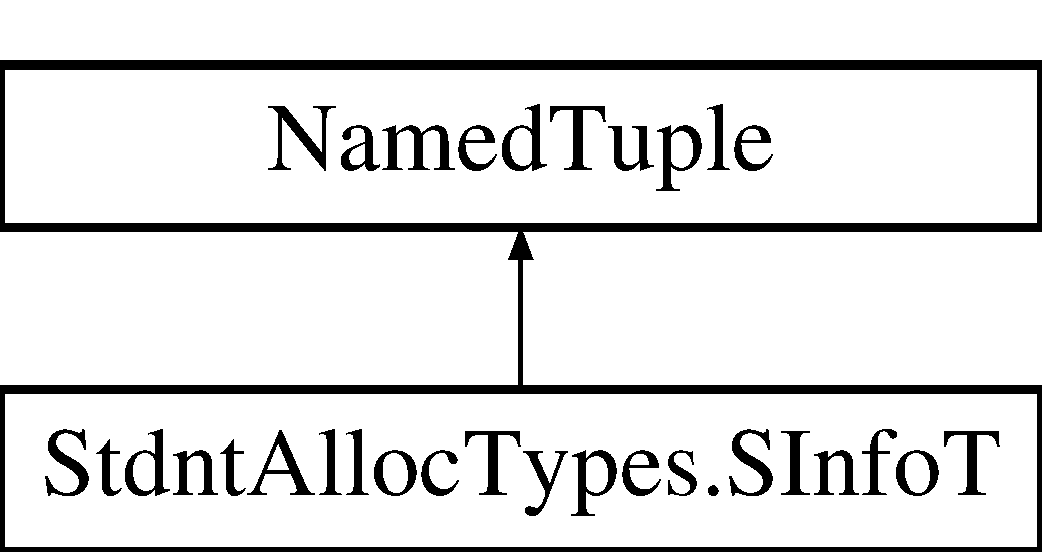
\includegraphics[height=2.000000cm]{class_stdnt_alloc_types_1_1_s_info_t}
\end{center}
\end{figure}


\subsection{Detailed Description}
A Named\+Tuple used to represent a student. 

A student has a\+: first name, last name, gender (given as a \hyperlink{class_stdnt_alloc_types_1_1_gen_t}{GenT} type), gpa, sequence of departments(given as a Seq\+A\+DT of \hyperlink{class_stdnt_alloc_types_1_1_dept_t}{DeptT}\textquotesingle{}s), and a boolean to represent if they have free choice. 

The documentation for this class was generated from the following file\+:\begin{DoxyCompactItemize}
\item 
src/\hyperlink{_stdnt_alloc_types_8py}{Stdnt\+Alloc\+Types.\+py}\end{DoxyCompactItemize}

\chapter{File Documentation}
\hypertarget{_a_a_lst_8py}{}\section{src/\+A\+A\+Lst.py File Reference}
\label{_a_a_lst_8py}\index{src/\+A\+A\+Lst.\+py@{src/\+A\+A\+Lst.\+py}}


Allocation Association List Module  


\subsection*{Classes}
\begin{DoxyCompactItemize}
\item 
class \hyperlink{class_a_a_lst_1_1_a_a_lst}{A\+A\+Lst.\+A\+A\+Lst}
\begin{DoxyCompactList}\small\item\em An abstract data type containing engineering departments and the students allocated into them. \end{DoxyCompactList}\end{DoxyCompactItemize}


\subsection{Detailed Description}
Allocation Association List Module 

\begin{DoxyAuthor}{Author}
Dominik Buszowiecki 
\end{DoxyAuthor}
\begin{DoxyDate}{Date}
February 9, 2019 
\end{DoxyDate}

\hypertarget{_d_cap_a_lst_8py}{}\section{src/\+D\+Cap\+A\+Lst.py File Reference}
\label{_d_cap_a_lst_8py}\index{src/\+D\+Cap\+A\+Lst.\+py@{src/\+D\+Cap\+A\+Lst.\+py}}


Department Capacity Association List  


\subsection*{Classes}
\begin{DoxyCompactItemize}
\item 
class \hyperlink{class_d_cap_a_lst_1_1_d_cap_a_lst}{D\+Cap\+A\+Lst.\+D\+Cap\+A\+Lst}
\begin{DoxyCompactList}\small\item\em An abstract data type containing the capacities of engineering departments as a list. \end{DoxyCompactList}\end{DoxyCompactItemize}


\subsection{Detailed Description}
Department Capacity Association List 

\begin{DoxyAuthor}{Author}
Dominik Buszowiecki 
\end{DoxyAuthor}
\begin{DoxyDate}{Date}
February 9, 2019 
\end{DoxyDate}

\hypertarget{_read_8py}{}\section{src/\+Read.py File Reference}
\label{_read_8py}\index{src/\+Read.\+py@{src/\+Read.\+py}}


Read  


\subsection*{Functions}
\begin{DoxyCompactItemize}
\item 
def \hyperlink{_read_8py_a7537be937b193ab3e5832bc901b00b90}{Read.\+load\+\_\+stdnt\+\_\+data}
\begin{DoxyCompactList}\small\item\em Loads students from a file into the S\+A\+Lst. \end{DoxyCompactList}\item 
def \hyperlink{_read_8py_ac54f5ecc26c145536f077f195df9f907}{Read.\+load\+\_\+dcap\+\_\+data}
\begin{DoxyCompactList}\small\item\em Loads department capacities from a file into the D\+Cap\+A\+Lst. \end{DoxyCompactList}\end{DoxyCompactItemize}


\subsection{Detailed Description}
Read 

\begin{DoxyAuthor}{Author}
Dominik Buszowiecki 
\end{DoxyAuthor}
\begin{DoxyDate}{Date}
February 9, 2019 
\end{DoxyDate}


\subsection{Function Documentation}
\mbox{\Hypertarget{_read_8py_file_ac54f5ecc26c145536f077f195df9f907}\label{_read_8py_file_ac54f5ecc26c145536f077f195df9f907}} 
\index{Read.\+py@{Read.\+py}!load\+\_\+dcap\+\_\+data@{load\+\_\+dcap\+\_\+data}}
\index{load\+\_\+dcap\+\_\+data@{load\+\_\+dcap\+\_\+data}!Read.\+py@{Read.\+py}}
\subsubsection{\texorpdfstring{load\+\_\+dcap\+\_\+data()}{load\_dcap\_data()}}
{\footnotesize\ttfamily def Read.\+load\+\_\+dcap\+\_\+data (\begin{DoxyParamCaption}\item[{}]{s }\end{DoxyParamCaption})}



Loads department capacities from a file into the D\+Cap\+A\+Lst. 

Each line in the file represents a department. The format of each line should be\+: ~\newline
 department\+\_\+name, capacity ~\newline
 where capacity is an integer. 
\begin{DoxyParams}{Parameters}
{\em s} & A string representing the name of the file \\
\hline
\end{DoxyParams}
\mbox{\Hypertarget{_read_8py_file_a7537be937b193ab3e5832bc901b00b90}\label{_read_8py_file_a7537be937b193ab3e5832bc901b00b90}} 
\index{Read.\+py@{Read.\+py}!load\+\_\+stdnt\+\_\+data@{load\+\_\+stdnt\+\_\+data}}
\index{load\+\_\+stdnt\+\_\+data@{load\+\_\+stdnt\+\_\+data}!Read.\+py@{Read.\+py}}
\subsubsection{\texorpdfstring{load\+\_\+stdnt\+\_\+data()}{load\_stdnt\_data()}}
{\footnotesize\ttfamily def Read.\+load\+\_\+stdnt\+\_\+data (\begin{DoxyParamCaption}\item[{}]{s }\end{DoxyParamCaption})}



Loads students from a file into the S\+A\+Lst. 

Each line in the file represents a student. The format of each line should be\+: ~\newline
 macid, firstname, lastname, gender, gpa, \mbox{[}choice1, choice2, ...\mbox{]}, freechoice ~\newline
 where gpa is a real number, gender is either male or female and freechoice is either True or False. 
\begin{DoxyParams}{Parameters}
{\em s} & A string representing the name of the file \\
\hline
\end{DoxyParams}

\hypertarget{_s_a_lst_8py}{}\section{src/\+S\+A\+Lst.py File Reference}
\label{_s_a_lst_8py}\index{src/\+S\+A\+Lst.\+py@{src/\+S\+A\+Lst.\+py}}


Student Association List  


\subsection*{Classes}
\begin{DoxyCompactItemize}
\item 
class \hyperlink{class_s_a_lst_1_1_s_a_lst}{S\+A\+Lst.\+S\+A\+Lst}
\begin{DoxyCompactList}\small\item\em An abstract data type of all first year engineerng students. \end{DoxyCompactList}\end{DoxyCompactItemize}


\subsection{Detailed Description}
Student Association List 

\begin{DoxyAuthor}{Author}
Dominik Buszowiecki 
\end{DoxyAuthor}
\begin{DoxyDate}{Date}
February 9, 2019 
\end{DoxyDate}

\hypertarget{_seq_a_d_t_8py}{}\section{src/\+Seq\+A\+DT.py File Reference}
\label{_seq_a_d_t_8py}\index{src/\+Seq\+A\+D\+T.\+py@{src/\+Seq\+A\+D\+T.\+py}}


Sequence A\+DT  


\subsection*{Classes}
\begin{DoxyCompactItemize}
\item 
class \hyperlink{class_seq_a_d_t_1_1_seq_a_d_t}{Seq\+A\+D\+T.\+Seq\+A\+DT}
\begin{DoxyCompactList}\small\item\em An abstract data type that represents a sequence of values. \end{DoxyCompactList}\end{DoxyCompactItemize}


\subsection{Detailed Description}
Sequence A\+DT 

\begin{DoxyAuthor}{Author}
Dominik Buszowiecki 
\end{DoxyAuthor}
\begin{DoxyDate}{Date}
February 9, 2019 
\end{DoxyDate}

\hypertarget{_stdnt_alloc_types_8py}{}\section{src/\+Stdnt\+Alloc\+Types.py File Reference}
\label{_stdnt_alloc_types_8py}\index{src/\+Stdnt\+Alloc\+Types.\+py@{src/\+Stdnt\+Alloc\+Types.\+py}}


Student Allocation Types  


\subsection*{Classes}
\begin{DoxyCompactItemize}
\item 
class \hyperlink{class_stdnt_alloc_types_1_1_gen_t}{Stdnt\+Alloc\+Types.\+GenT}
\begin{DoxyCompactList}\small\item\em An Enumerated type of possible genders \end{DoxyCompactList}\item 
class \hyperlink{class_stdnt_alloc_types_1_1_dept_t}{Stdnt\+Alloc\+Types.\+DeptT}
\begin{DoxyCompactList}\small\item\em An Enumerated type of possible engineering departments. \end{DoxyCompactList}\item 
class \hyperlink{class_stdnt_alloc_types_1_1_s_info_t}{Stdnt\+Alloc\+Types.\+S\+InfoT}
\begin{DoxyCompactList}\small\item\em A Named\+Tuple used to represent a student. \end{DoxyCompactList}\end{DoxyCompactItemize}


\subsection{Detailed Description}
Student Allocation Types 

\begin{DoxyAuthor}{Author}
Dominik Buszowiecki 
\end{DoxyAuthor}
\begin{DoxyDate}{Date}
February 9, 2019 
\end{DoxyDate}

%--- End generated contents ---

% Index
\backmatter
\newpage
\phantomsection
\clearemptydoublepage
\addcontentsline{toc}{chapter}{Index}
\printindex

\end{document}
